\documentclass[11pt]{article}
\usepackage[margin=1in]{geometry}
\usepackage{amsmath,amssymb,bm}
\usepackage{booktabs}
\usepackage{enumitem}
\usepackage{graphicx}
\usepackage[hidelinks]{hyperref}
\usepackage{microtype}

\title{Runaway Probability Neural Model Development}
\author{}
\date{September 2026}

\newcommand{\RPF}{P}
\newcommand{\xiCoord}{\xi}
\newcommand{\param}{\boldsymbol{\lambda}}

\begin{document}
\maketitle

\begin{abstract}
This report documents development of a JAX-trained neural model for the steady
relativistic runaway-electron first-passage probability.  The project begins
with a vanilla supervised model and adds architectural, numerical, and
physics-informed features only after each simpler stage is measured.
\end{abstract}

\tableofcontents
\newpage

\section{Purpose and terminology}

The target is a bounded response function
\begin{equation}
  0 \leq \RPF(p,\xiCoord;\param) \leq 1,
\end{equation}
where $p$ is dimensionless momentum, $\xiCoord$ is pitch cosine, and
$\param$ contains plasma and field parameters.

\emph{Neural model} is the general term used in this report.  JAX provides
the numerical and automatic-differentiation framework used to train models.
\emph{Physics-informed neural network} (PINN) refers only to a training mode
that includes a physics residual or boundary constraints in its objective.
Supervised data-driven training is a neural-model baseline, not automatically
a PINN.

\section{Scientific problem}

The model estimates first-passage probability for an electron evolving in a
relativistic kinetic system.  The successful event is exit through the upper
momentum boundary; failure is exit through the lower-momentum boundary.
The response depends on seven physical parameters:
\begin{equation}
  \param = (E/E_c,\; T_e,\; n_D,\; n_{Ne},\; z_D,\; z_{Ne},\; B).
\end{equation}

The CPU finite-volume solver defines reference labels.  Neural models learn
an approximation to those labels or to the governing normalized residual,
depending on training mode.

\section{Reference finite-volume data}

The reference solver uses a conservative finite-volume discretization of the
kinetic operator and a volume-weighted discrete adjoint.  The dataset pipeline
performs the following operations:
\begin{enumerate}[nosep]
  \item Generate reproducible Sobol parameter cases.
  \item Build composite momentum grids with upper-tail concentration for
        near-threshold cases.
  \item Solve the sparse adjoint first-passage system on CPU.
  \item Add an analytic zero-probability low-momentum tail.
  \item Reject trivial or invalid cases.
  \item Store exact cell centers, fields, metadata, and checksums.
\end{enumerate}

Finite-volume labels remain outside JAX automatic differentiation.  This
separation keeps reference-label generation independent from model training.
The current dataset contains 131072 cases on a coarsened $232\times44$
phase-space grid.  Boundary-adjacent cells are retained during coarsening so
the upper-momentum success boundary is not discarded.

\begin{figure}[ht]
  \centering
  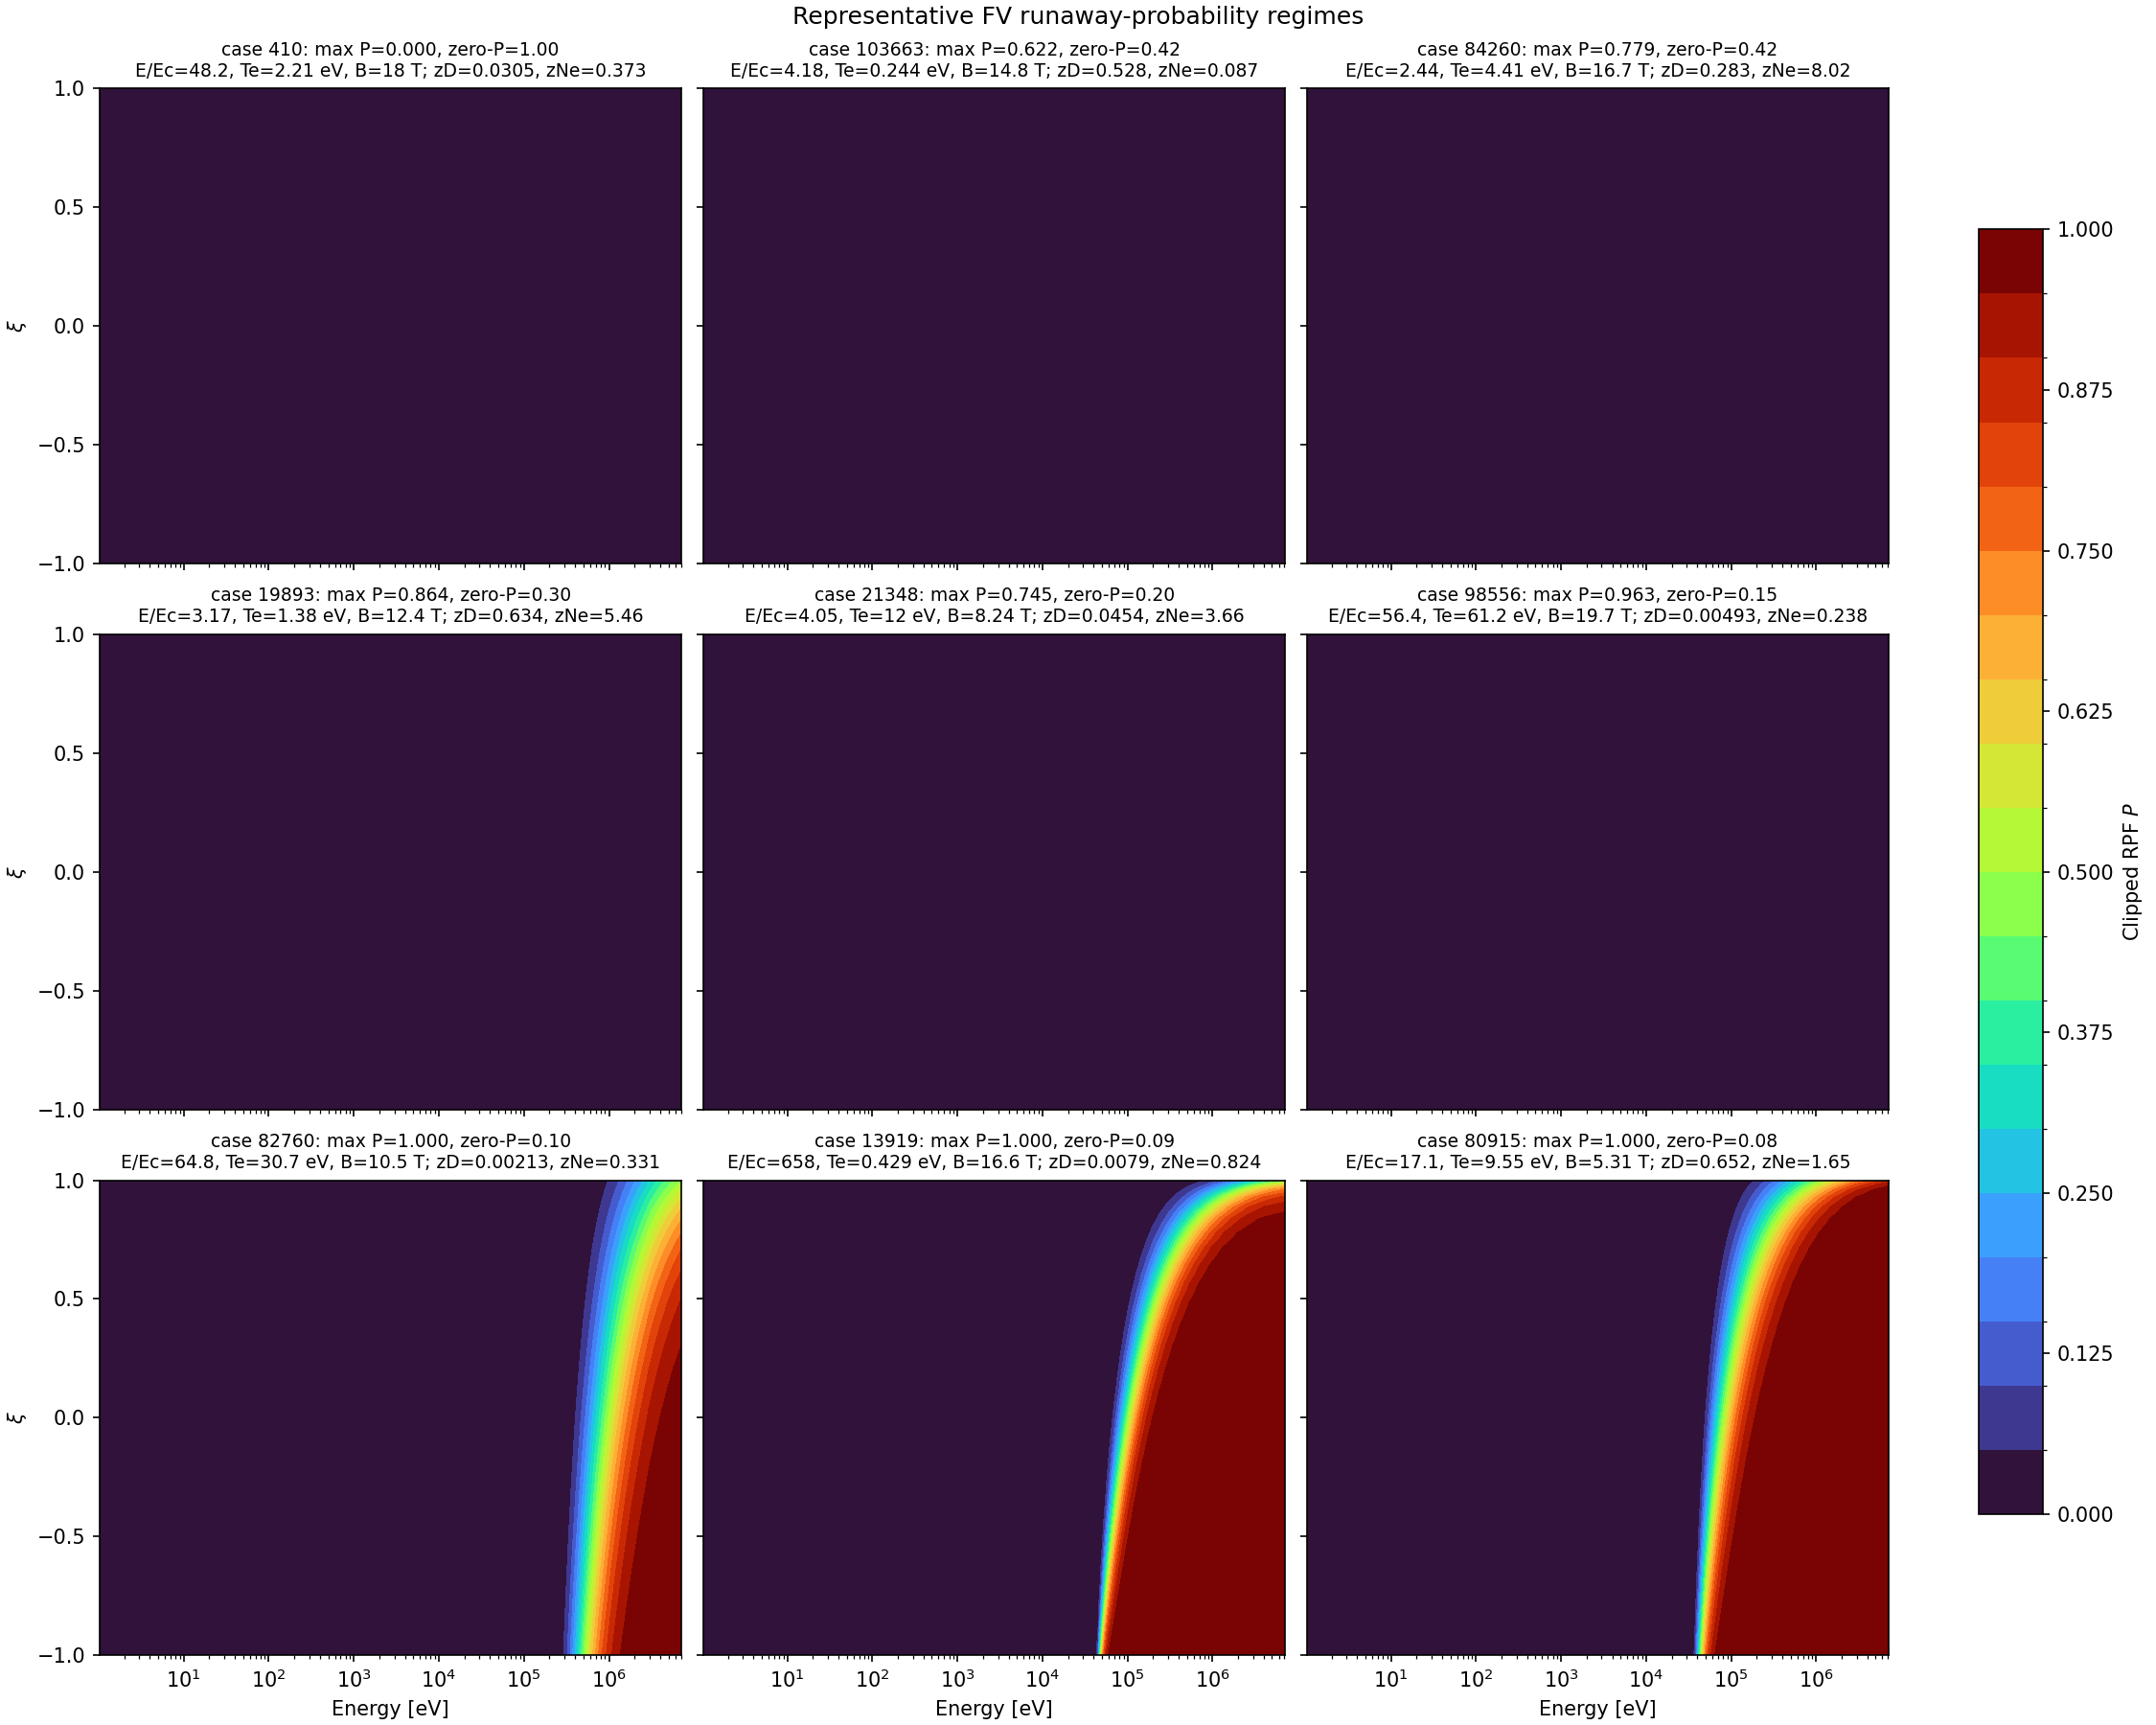
\includegraphics[width=0.98\textwidth]{figures/rpf_regime_probes.png}
  \caption{Representative clipped FV RPF solutions across selected physical regimes.}
  \label{fig:rpf-regimes}
\end{figure}

\section{Normalized model interface}

The pointwise model input has nine normalized coordinates:
\begin{equation}
  z = (z_p, z_\xi, z_{E/E_c}, z_{T_e}, z_{n_D}, z_{n_{Ne}}, z_{z_D}, z_{z_{Ne}}, z_B).
\end{equation}

The first two coordinates represent phase space.  The remaining seven represent
the physical parameter case.  Logarithmic mappings are used for positive
quantities where appropriate.  All model calculations use FP64.

\subsection{Initial production domain}

The initial production configuration defines the following parameter ranges.
The JSON files remain operational run definitions; this table records the
domain used by the current model-development baseline.

\begin{center}
\begin{tabular}{lrrl}
\toprule
Parameter & Minimum & Maximum & Mapping \\
\midrule
$E/E_c$ & $1$ & $1000$ & logarithmic \\
$T_e$ [eV] & $0.1$ & $100$ & logarithmic \\
$n_D$ [m$^{-3}$] & $10^{20}$ & $10^{22}$ & logarithmic \\
$n_{Ne}$ [m$^{-3}$] & $10^{16}$ & $10^{22}$ & logarithmic \\
$z_D$ & $0.001$ & $1$ & logarithmic \\
$z_{Ne}$ & $0.001$ & $10$ & logarithmic \\
$B$ [T] & $1$ & $20$ & linear \\
\bottomrule
\end{tabular}
\end{center}

The phase-space domain uses $p\in[0.002,15]$ and $\xiCoord\in[-1,1]$.
Charge-state means use $z_D,z_{Ne}\geq0.001$ to sample sub-unity states
without reaching zero-electron singularities. Domain validation enforces
positive ordered bounds and matching
parameter ranges across FV and neural-model configurations.

\begin{figure}[ht]
  \centering
  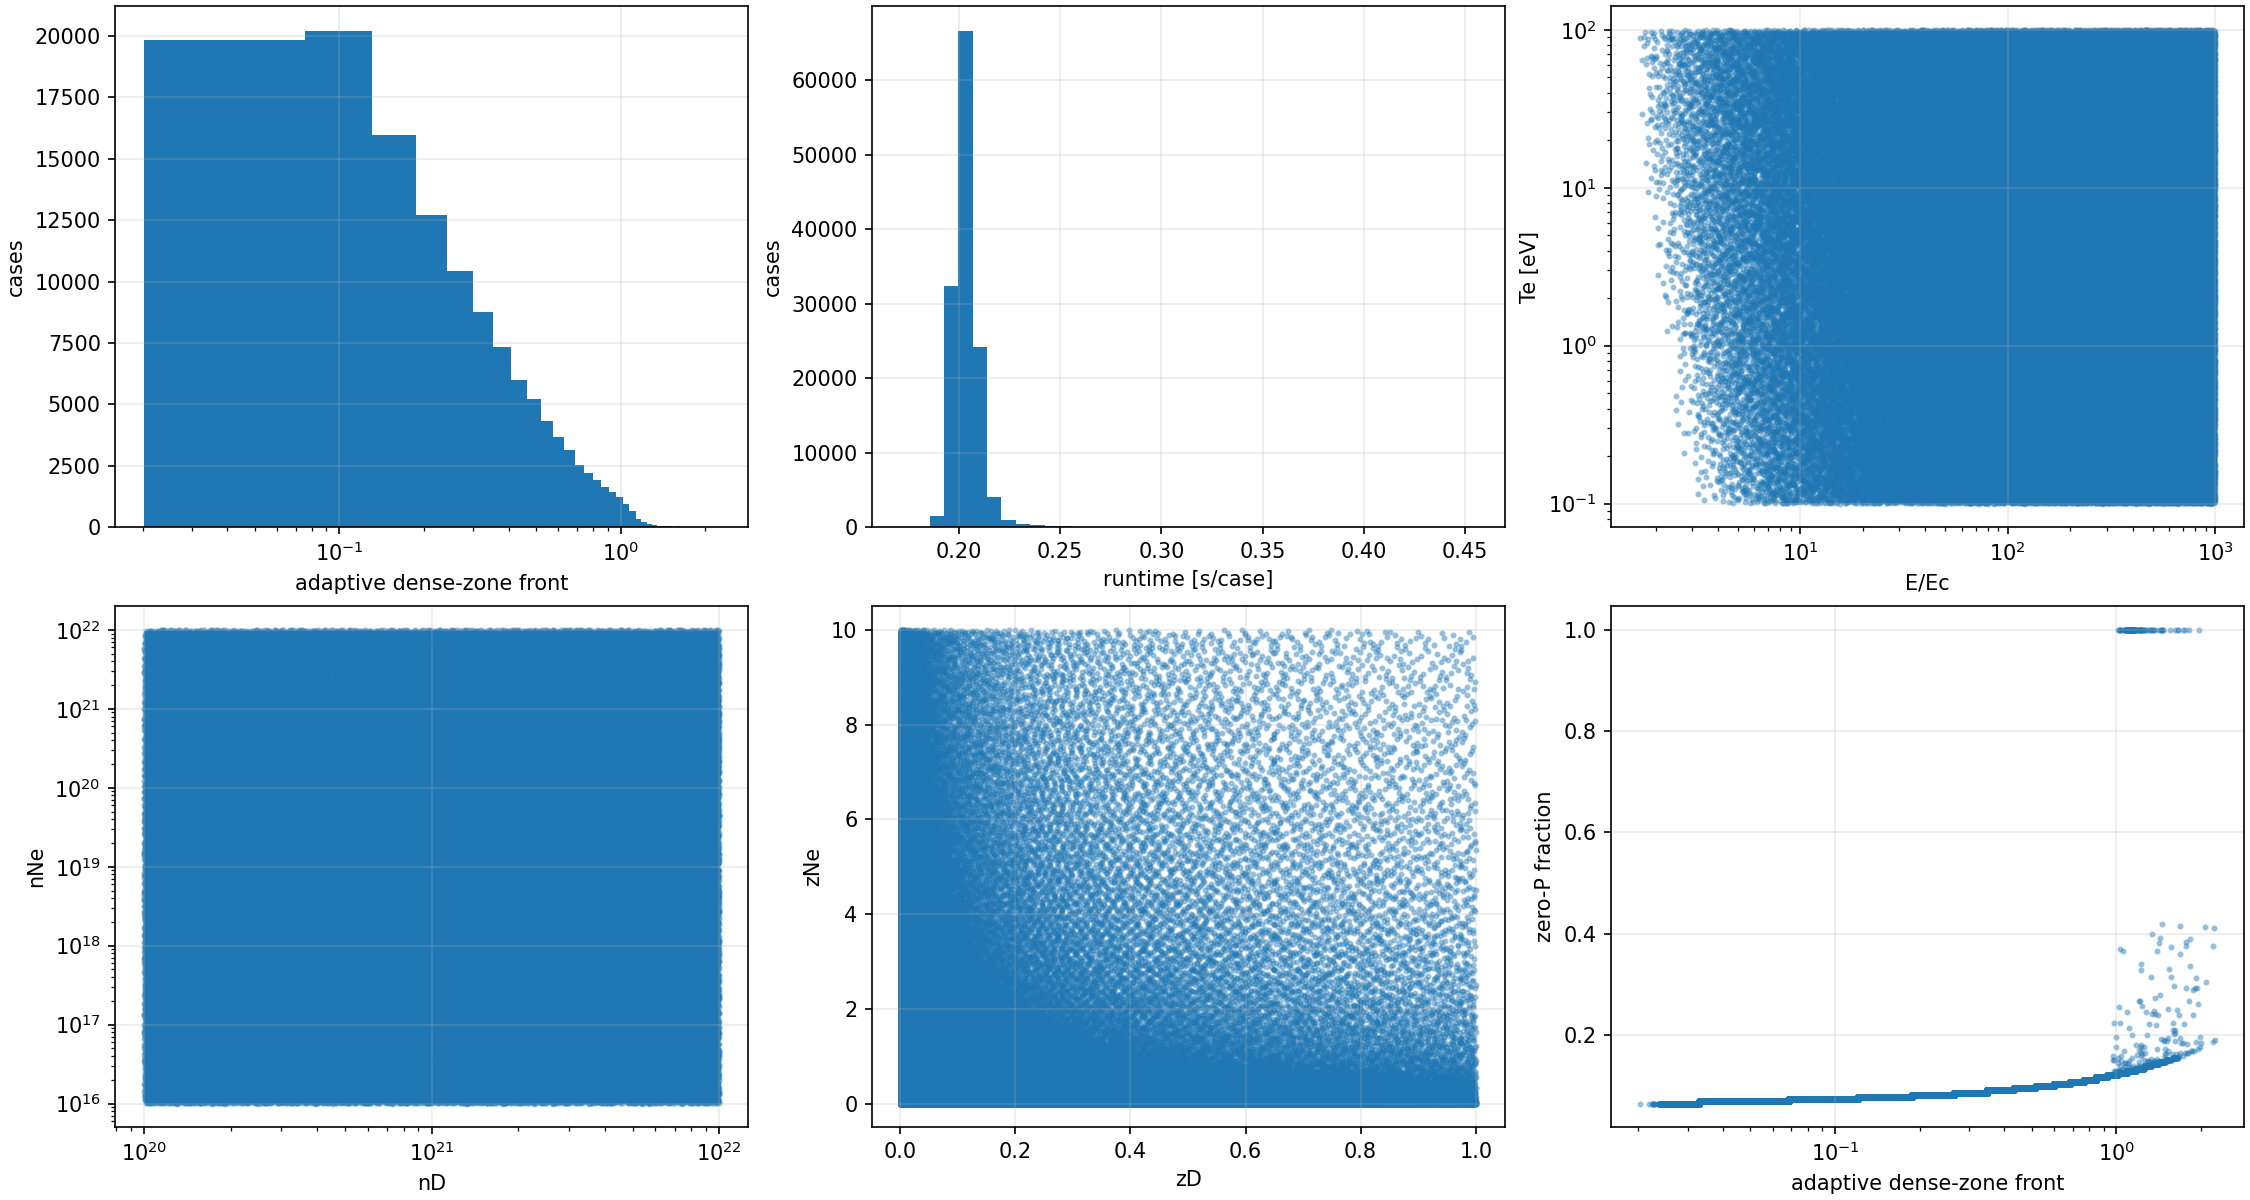
\includegraphics[width=0.98\textwidth]{figures/parameter_coverage_scatter.png}
  \caption{FV dataset coverage and solver-runtime diagnostics generated by the dataset analysis routine.}
  \label{fig:parameter-coverage}
\end{figure}

\section{Model development sequence}

Development proceeds from the smallest useful baseline toward more structured
models:

\begin{enumerate}
  \item \textbf{Vanilla MLP.} Train a pointwise MLP with supervised FV labels.
  \item \textbf{Baseline measurements.} Record train/test error, regional
        error, probability bounds, and reproducibility across seeds.
  \item \textbf{Output constraints.} Compare bounded output transforms and
        low-momentum behavior.
  \item \textbf{Architecture growth.} Test wider/deeper MLPs and, when useful,
        a DeepONet representation separating parameter and phase-space inputs.
  \item \textbf{Physics-informed training.} Add PDE, threshold, and boundary
        terms only after the supervised baseline is understood.
  \item \textbf{Active acquisition.} Use residual ranking to request new CPU
        FV labels only after fixed-data behavior is qualified.
\end{enumerate}

Each stage must preserve a clear comparison with the previous stage.  Added
complexity is justified by measured improvement, not by architecture alone.

\section{Initial vanilla experiment}

The first experiment uses supervised FV data with a pointwise MLP.  The model
has width $128$, six hidden layers, nine input coordinates, and a sigmoid
output transform.  SOAP uses $\beta_1=\beta_2=0.997$, zero weight decay, an
initial learning rate of $10^{-3}$, cosine decay to a final fraction of $0.1$,
and a global batch size of $131072$.

Training uses an 80/20 parameter-case split, 5000 optimizer steps, and 16
A100 GPUs across four nodes.  Checkpoints are written at steps 1000, 2000,
3000, 4000, and 5000; the loss history also records the initial step.

The run uses 104858 training cases and 26214 test cases.  Initial results are:
\begin{center}
\begin{tabular}{lr}
\toprule
Metric & Value \\
\midrule
Training MSE & $7.84742\times10^{-5}$ \\
Test MSE & $1.53796\times10^{-4}$ \\
\bottomrule
\end{tabular}
\end{center}

These results define the first baseline for later architecture and
physics-informed comparisons.

\begin{figure}[ht]
  \centering
  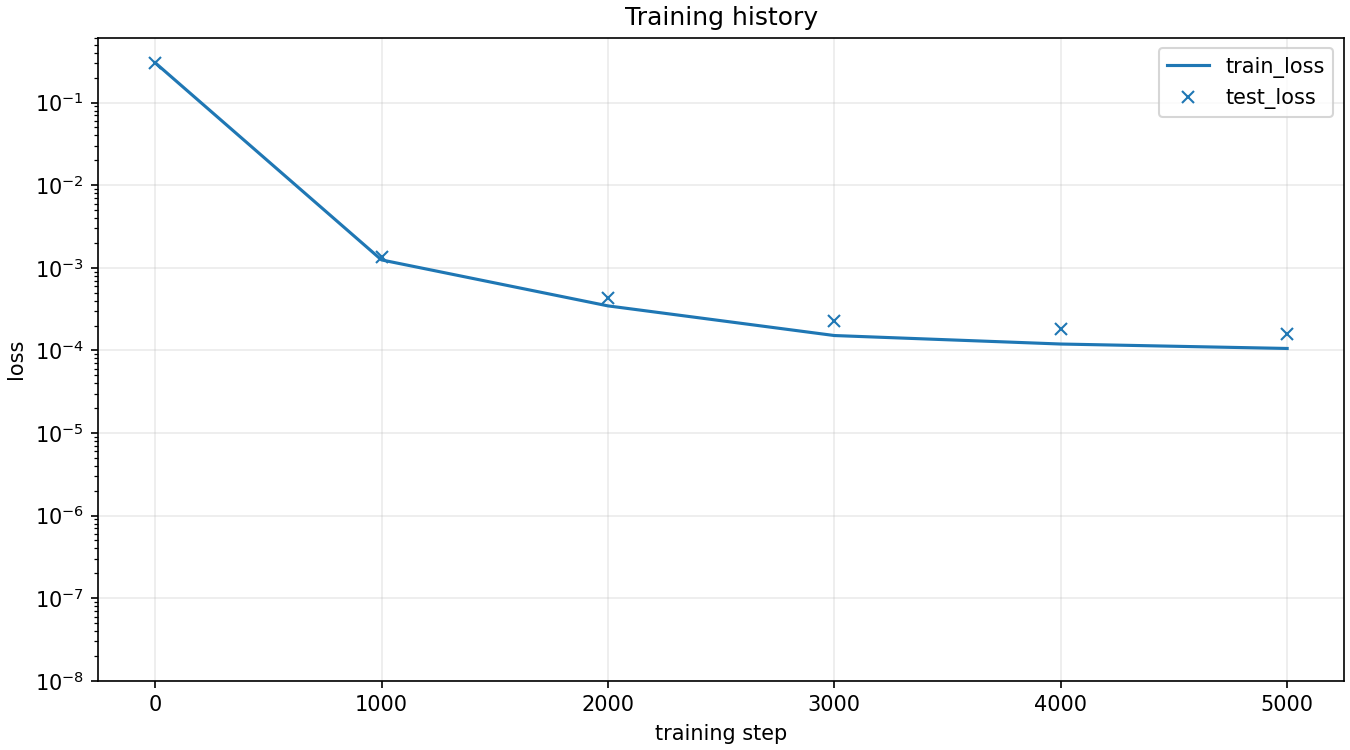
\includegraphics[width=0.82\textwidth]{figures/loss_history.png}
  \caption{Training and test loss history for the vanilla MLP.}
  \label{fig:loss-history}
\end{figure}

\subsection{Validation results}

The trained model was evaluated against all 131072 generated FV cases, or
1337982976 exact FV cells.  Validation used the completed model and dataset
manifests before computing predictions and residuals.

\begin{center}
\begin{tabular}{lr}
\toprule
Metric & Value \\
\midrule
Validation MSE & $1.00219\times10^{-4}$ \\
Maximum absolute error & $9.87202\times10^{-1}$ \\
PDE residual RMS & $4.28710\times10^{-2}$ \\
\bottomrule
\end{tabular}
\end{center}

The regional MSE is $1.45221\times10^{-5}$ in the zero-probability region,
$1.79634\times10^{-4}$ in the transition region, and
$3.56743\times10^{-7}$ in the saturated region.  The largest errors occur
near the transition boundary.

\begin{figure}[p]
  \centering
  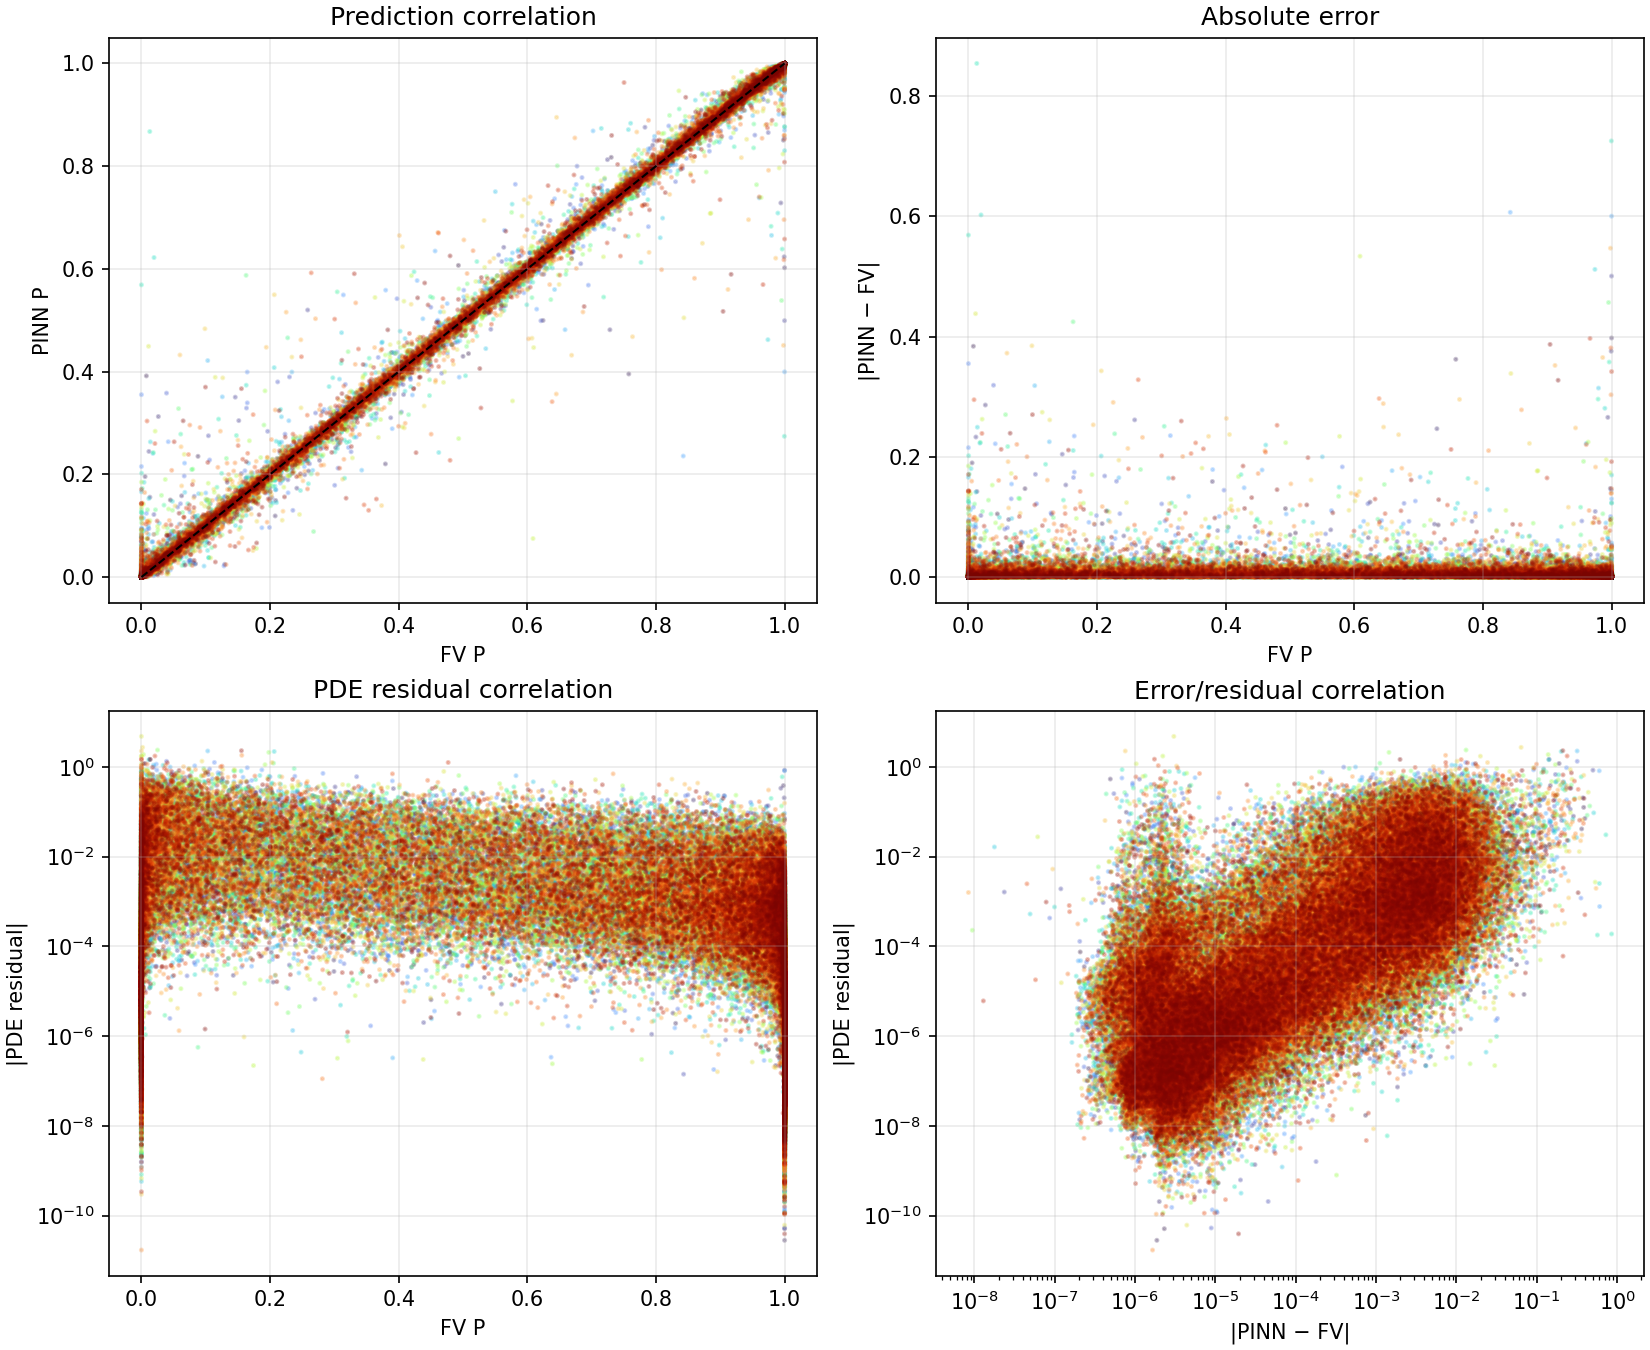
\includegraphics[width=0.98\textwidth]{figures/validation_correlation.png}
  \caption{Vanilla MLP validation correlation, absolute error, and PDE residuals.}
  \label{fig:validation-correlation}
\end{figure}

\begin{figure}[p]
  \centering
  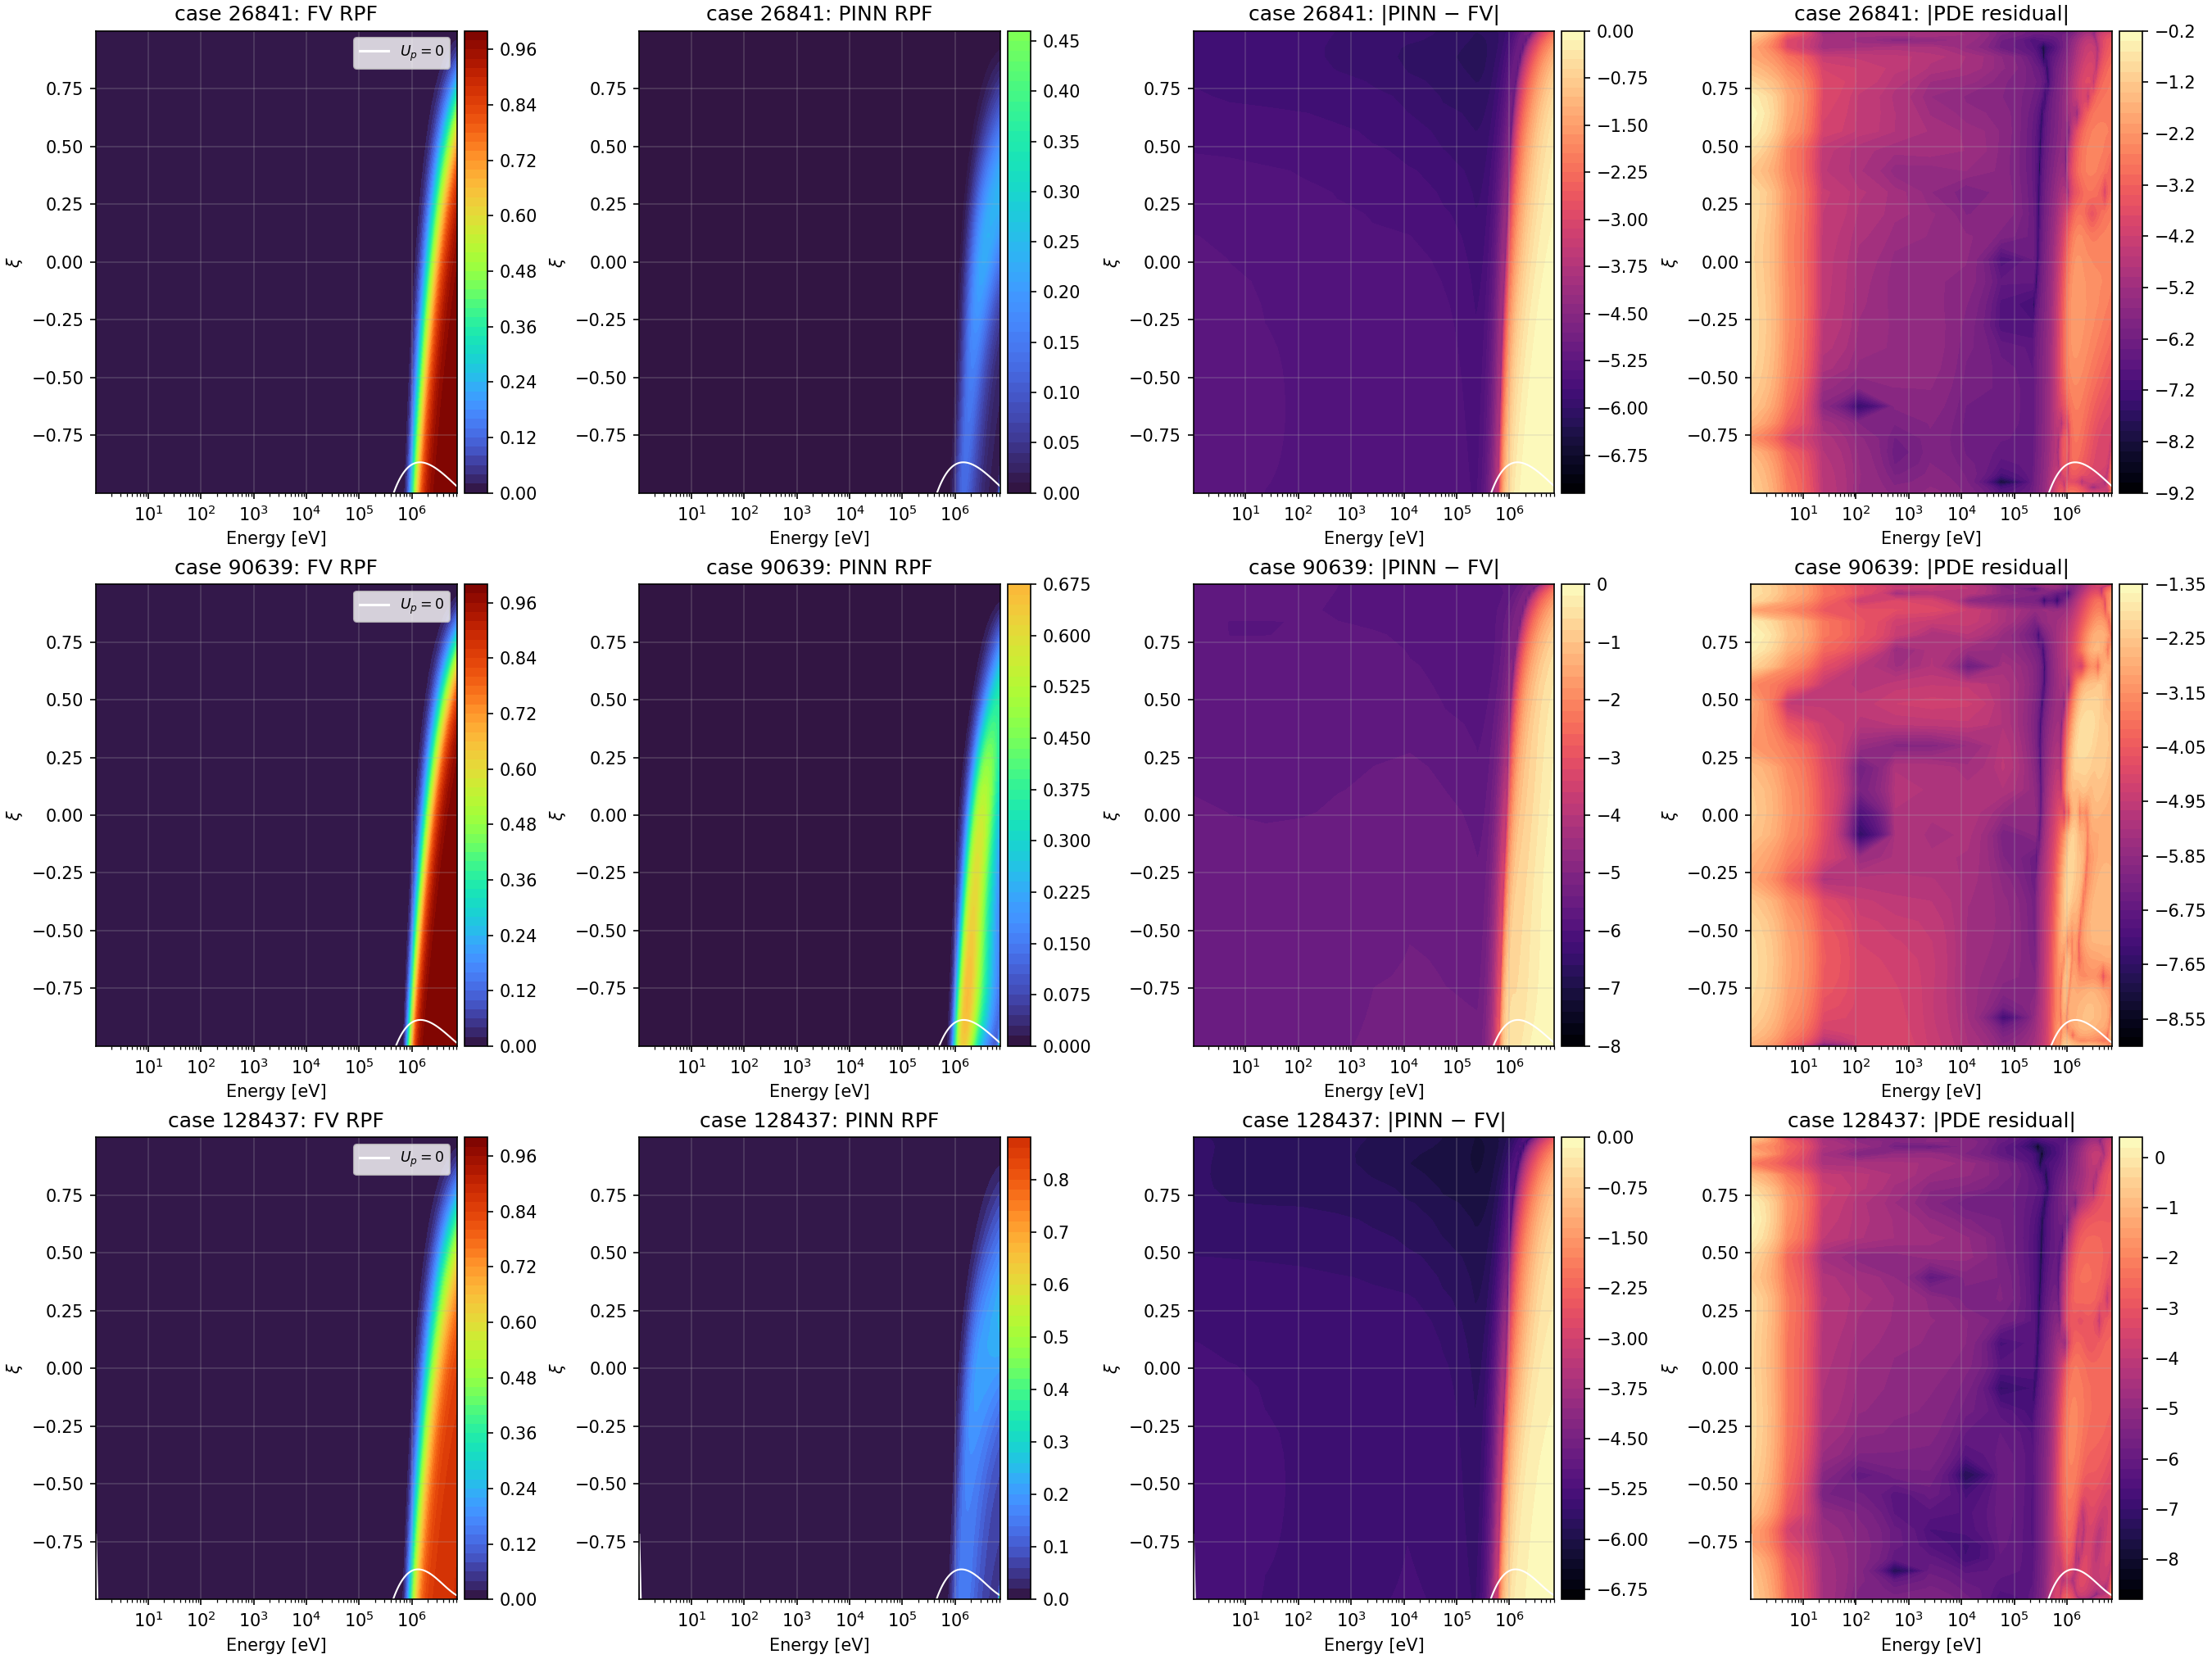
\includegraphics[width=0.98\textwidth]{figures/validation_cases.png}
  \caption{Representative worst-error validation cases from the vanilla MLP.}
  \label{fig:validation-cases}
\end{figure}

\section{Data-plus-physics experiment}

The second experiment uses the corrected composite-grid dataset while keeping
the same MLP, SOAP optimizer, and
16-GPU allocation, then adds the PDE residual to the data objective.  The PDE
loss uses the same 65536 training FV input coordinates, so no separate
collocation set is introduced.  The data-loss weight is $1$ and the PDE-loss
weight is $10^{-3}$; threshold, low-momentum, and high-momentum boundary losses
remain disabled.

\begin{center}
\begin{tabular}{lr}
\toprule
Metric & Value \\
\midrule
Training MSE & $6.11134\times10^{-4}$ \\
Test MSE & $1.83293\times10^{-3}$ \\
Validation MSE & $1.73581\times10^{-3}$ \\
Validation maximum absolute error & $9.98960\times10^{-1}$ \\
Validation PDE residual RMS & $5.47506\times10^{2}$ \\
\bottomrule
\end{tabular}
\end{center}

This weighting substantially worsens supervised prediction relative to
the data-only baseline.  The result indicates that PDE weighting and residual
normalization need tuning before drawing a physics-benefit conclusion.

\begin{figure}[ht]
  \centering
  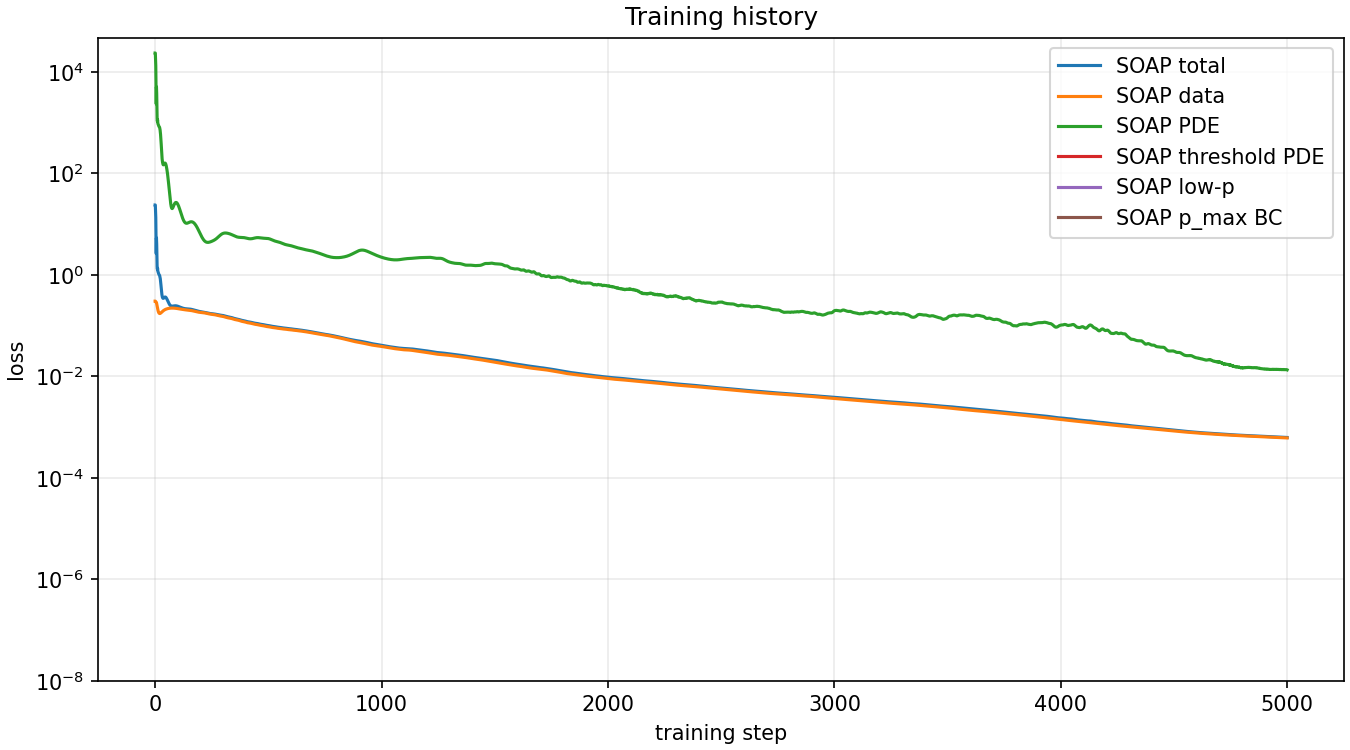
\includegraphics[width=0.82\textwidth]{figures/loss_history_data_physics.png}
  \caption{Training and test loss history for data-plus-physics training.}
  \label{fig:loss-history-data-physics}
\end{figure}

\begin{figure}[p]
  \centering
  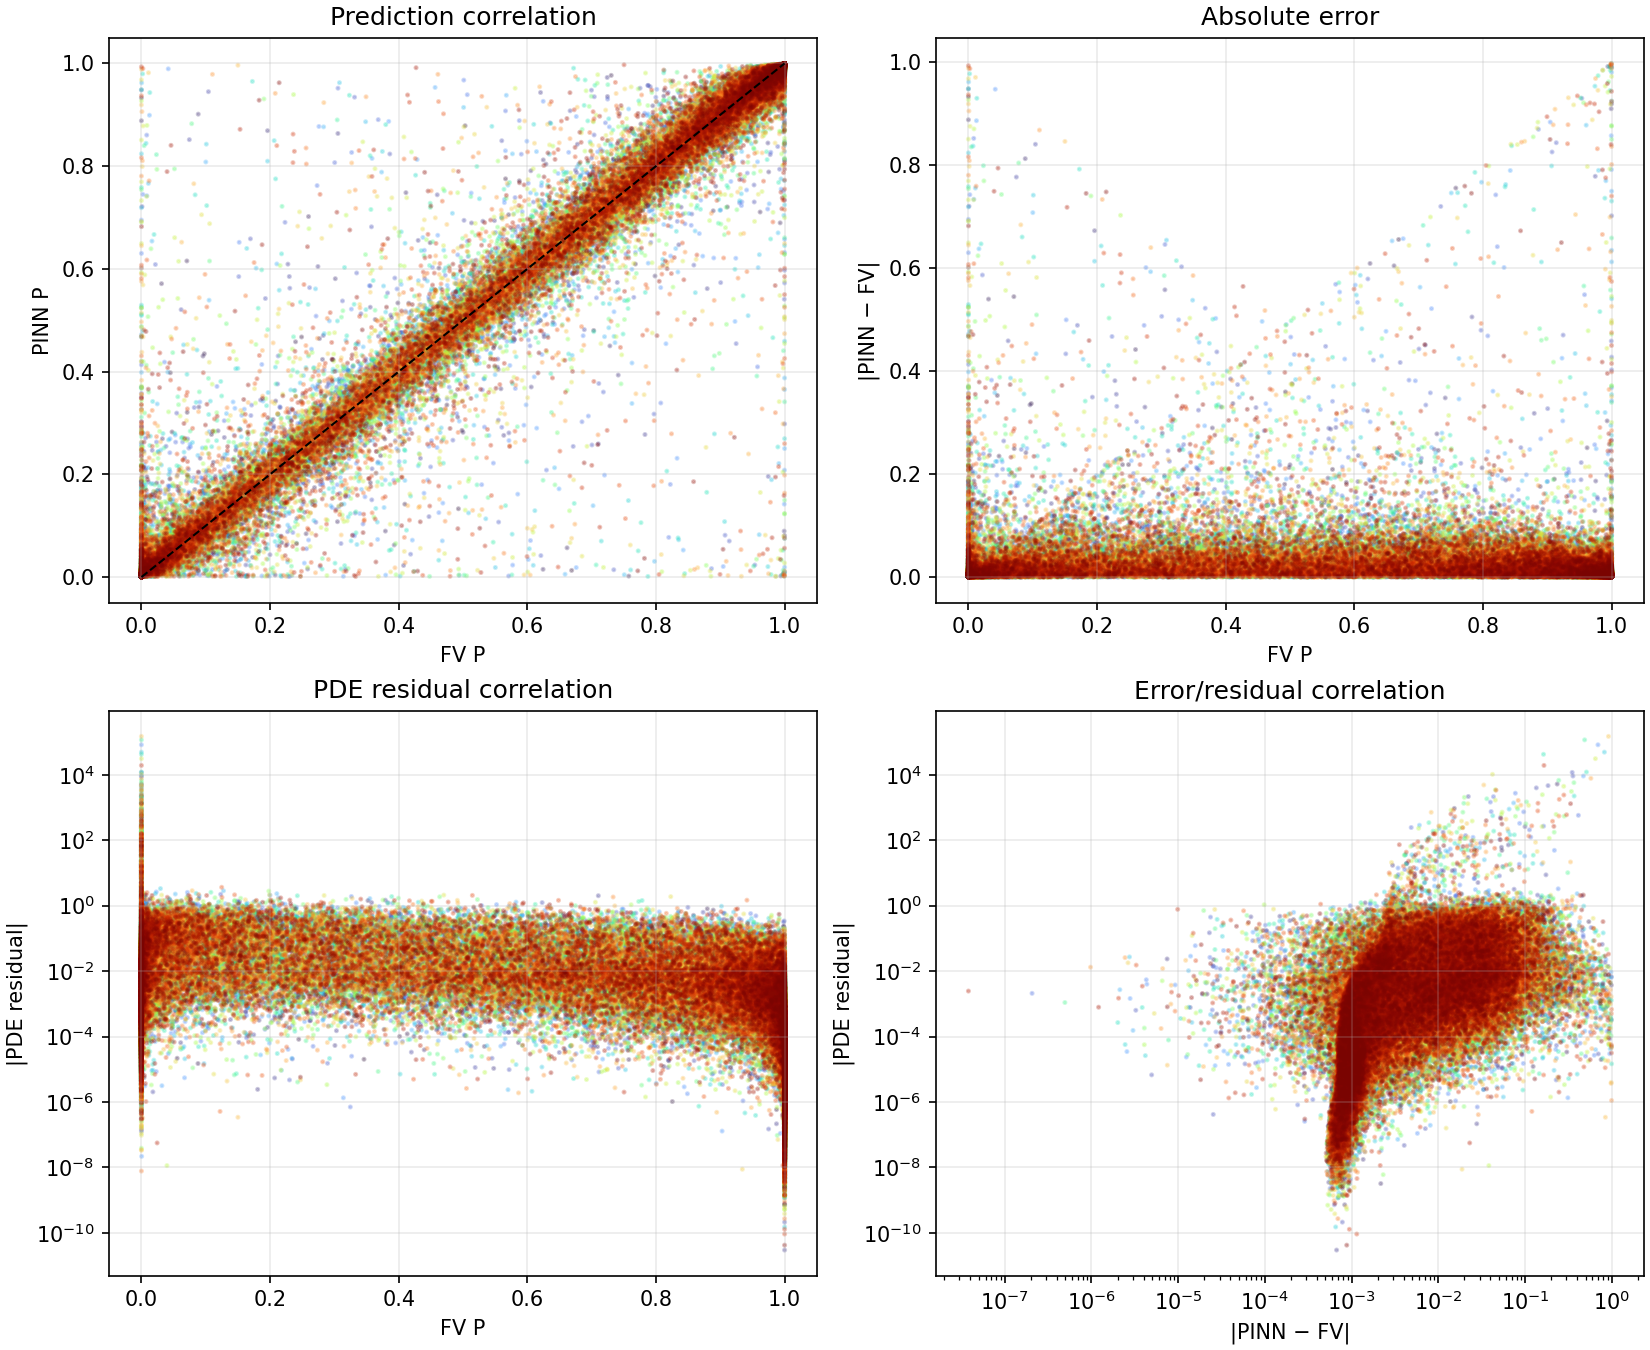
\includegraphics[width=0.98\textwidth]{figures/validation_correlation_data_physics.png}
  \caption{Data-plus-physics validation correlation, absolute error, and PDE residuals.}
  \label{fig:validation-correlation-data-physics}
\end{figure}

\begin{figure}[p]
  \centering
  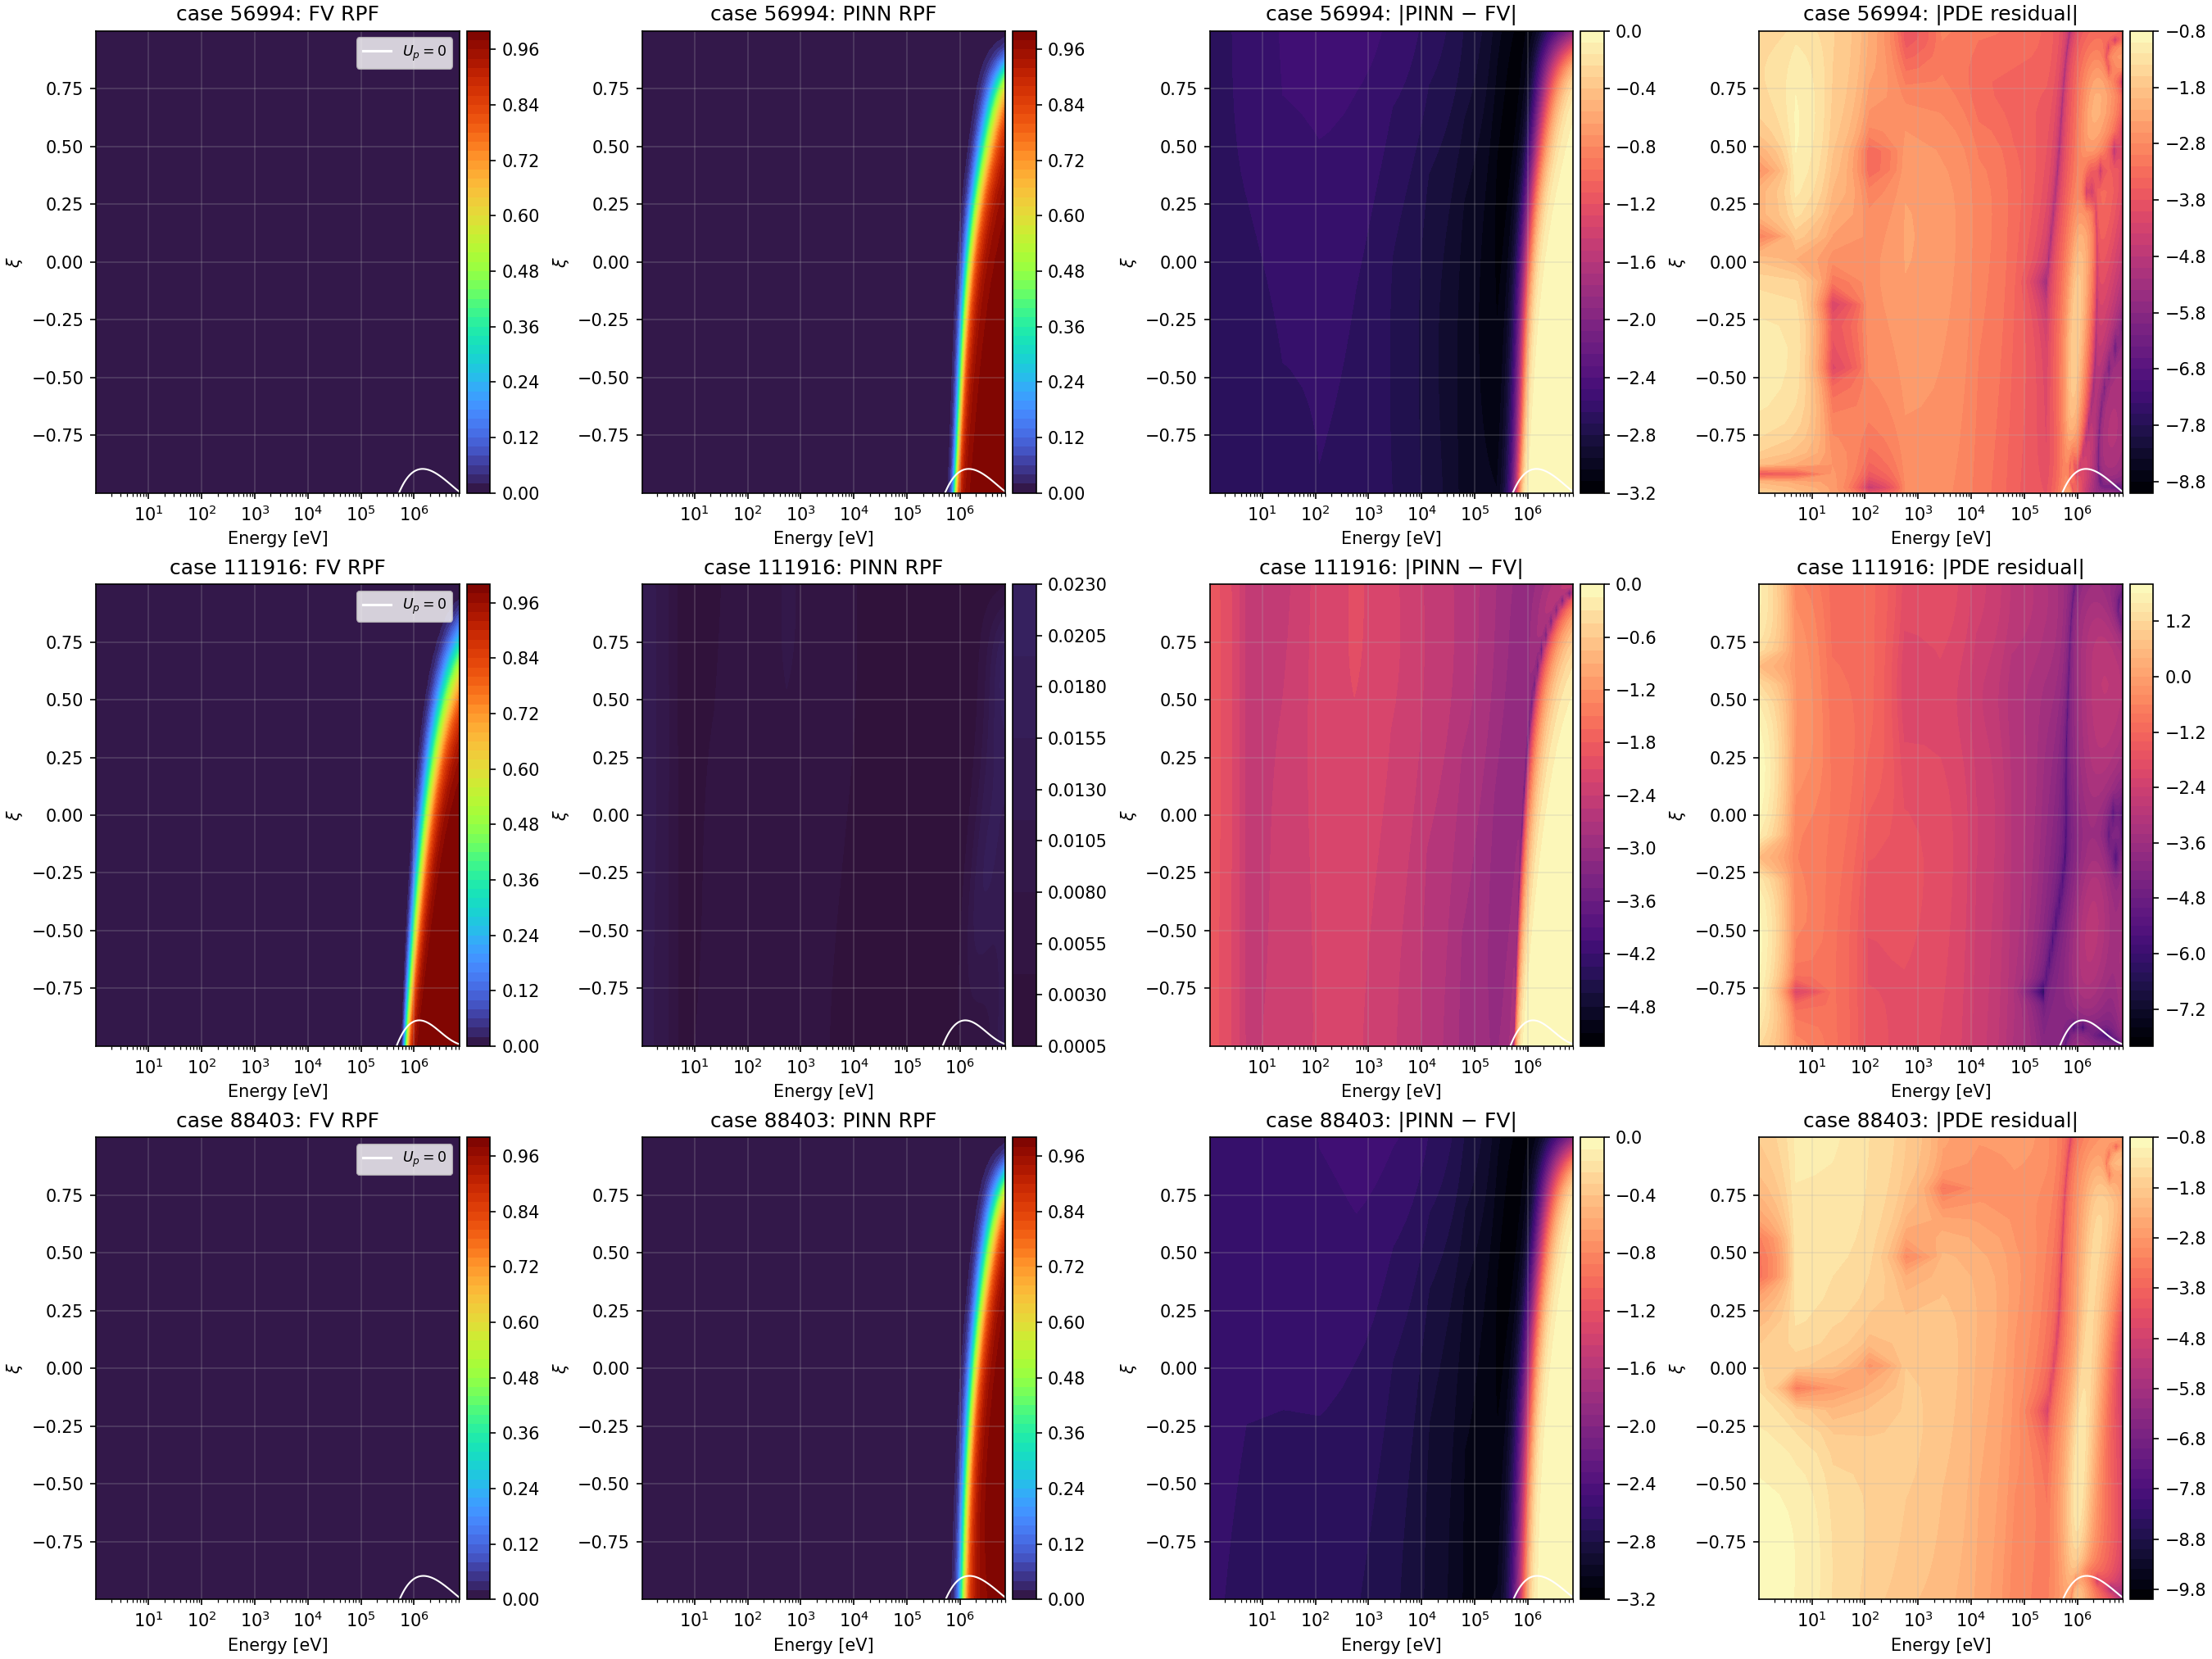
\includegraphics[width=0.98\textwidth]{figures/validation_cases_data_physics.png}
  \caption{Representative worst-error validation cases from data-plus-physics training.}
  \label{fig:validation-cases-data-physics}
\end{figure}

\section{Earlier data-plus-physics with exact upper-boundary loss}

The earlier third experiment retained the data-plus-PDE setup and enabled the exact
upper-momentum success boundary loss.  It uses 16384 boundary collocation
points, boundary-loss weight $1$, data-loss weight $1$, and PDE-loss weight
$10^{-3}$.  This run predates the corrected composite-grid dataset and has not
been rerun here.  The boundary targets are evaluated at $p=p_{\max}$ using the
outward-drift success condition.

\begin{center}
\begin{tabular}{lr}
\toprule
Metric & Value \\
\midrule
Training MSE & $2.75380\times10^{-3}$ \\
Test MSE & $3.59397\times10^{-3}$ \\
Validation MSE & $3.46047\times10^{-3}$ \\
Validation maximum absolute error & $9.98953\times10^{-1}$ \\
Validation PDE residual RMS & $1.12364\times10^{2}$ \\
\bottomrule
\end{tabular}
\end{center}

This boundary-weighted configuration does not improve the initial hybrid
baseline.  Boundary-loss weighting and PDE normalization require further
tuning before this objective can be judged beneficial.

\begin{figure}[ht]
  \centering
  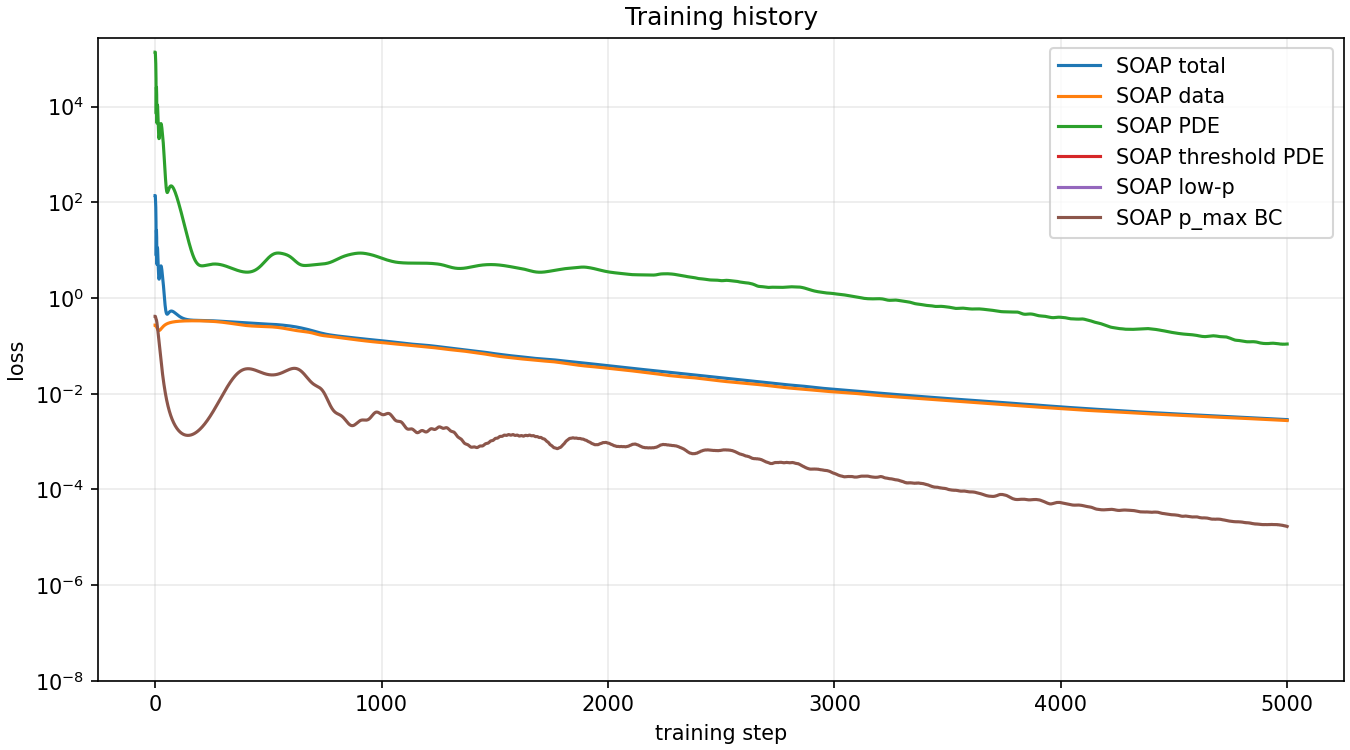
\includegraphics[width=0.82\textwidth]{figures/loss_history_data_physics_boundary.png}
  \caption{Training and test loss history with upper-boundary loss.}
  \label{fig:loss-history-data-physics-boundary}
\end{figure}

\begin{figure}[p]
  \centering
  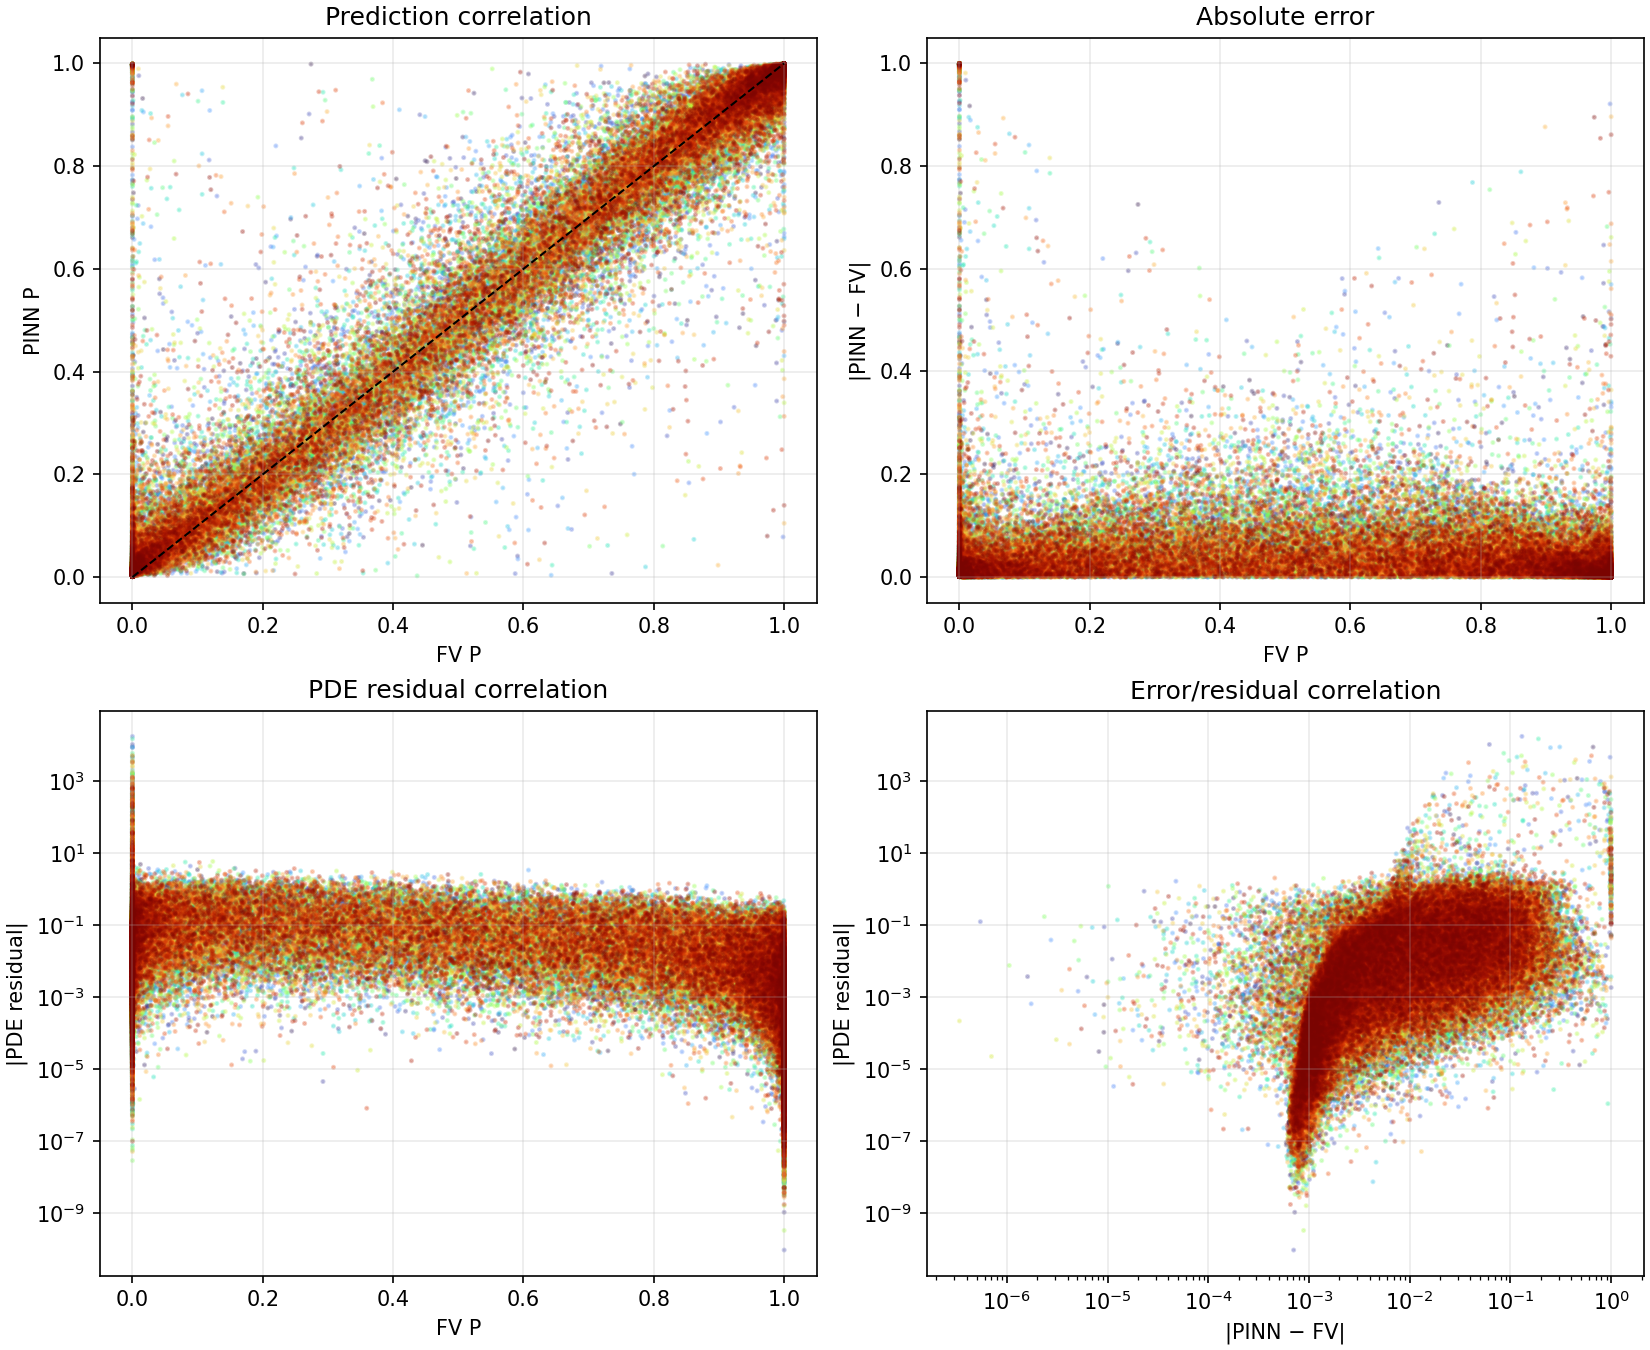
\includegraphics[width=0.98\textwidth]{figures/validation_correlation_data_physics_boundary.png}
  \caption{Boundary-loss validation correlation, absolute error, and PDE residuals.}
  \label{fig:validation-correlation-data-physics-boundary}
\end{figure}

\begin{figure}[p]
  \centering
  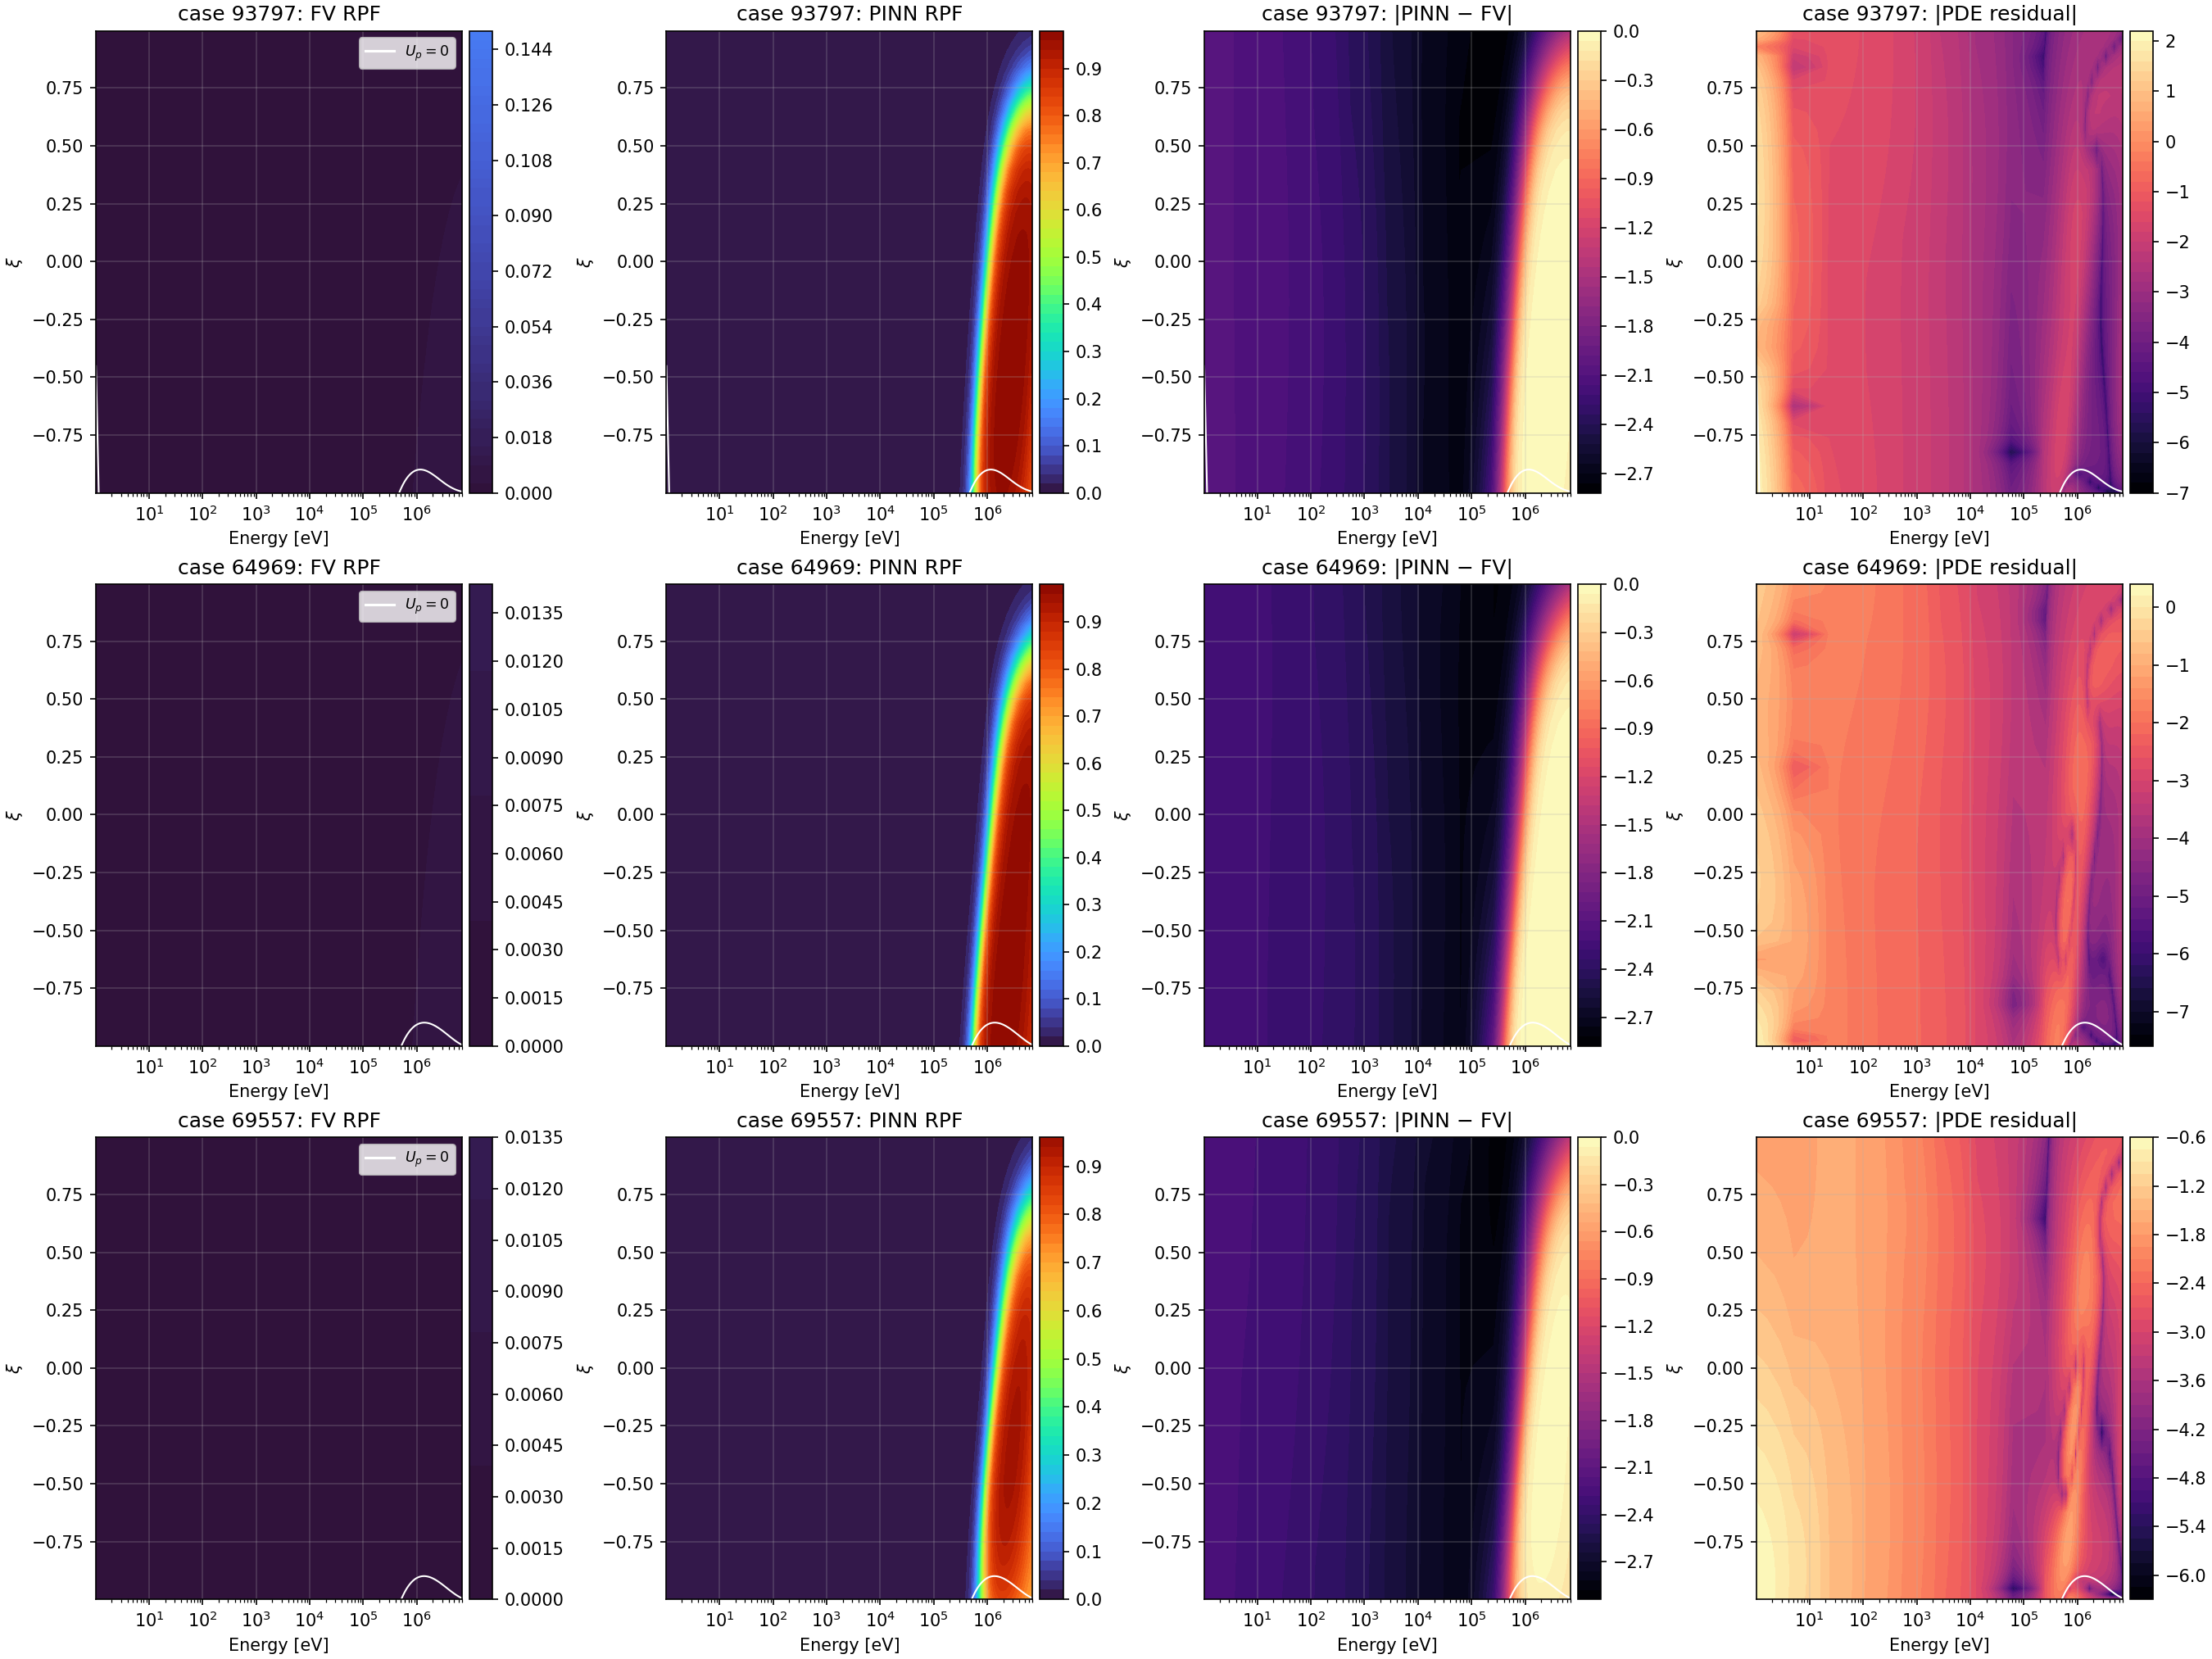
\includegraphics[width=0.98\textwidth]{figures/validation_cases_data_physics_boundary.png}
  \caption{Representative validation cases with upper-boundary loss.}
  \label{fig:validation-cases-data-physics-boundary}
\end{figure}

\section{Training modes}

\subsection{Supervised data mode}

The model minimizes error between neural predictions and FV probabilities.
Cases split at parameter-case level, not individual cells, so test cases
measure interpolation across physical parameter space.

\subsection{Physics-informed mode}

The model objective may combine FV data loss, normalized PDE residual loss,
threshold residual loss, low-momentum loss, and upper-boundary success loss.
The term ``PINN'' applies to this mode because automatic differentiation
contributes physics residuals to training.

\subsection{Active training}

The model ranks candidate points by PDE residual.  Selected parameter cases
are solved by the CPU FV pipeline, then appended to the training data.  FV
acquisition remains outside JAX differentiation.

\section{Evaluation protocol}

Every model stage should report:
\begin{itemize}[nosep]
  \item global MSE and maximum absolute error;
  \item error in zero, transition, and saturated probability regions;
  \item PDE residual statistics when physics terms are active;
  \item per-case metrics on held-out parameter cases;
  \item model, dataset, configuration, and environment identifiers.
\end{itemize}

Validation must verify completed manifests and checksums before analytics.
Production generation, training, and validation run inside Slurm allocations.

\section{Reproducibility contract}

Production runs use the project-local environment, explicit JSON
configuration, fixed Sobol seeds, FP64 JAX settings, fresh artifact paths,
and atomic manifest publication.  Generated datasets, models, checkpoints,
histories, and validation outputs are run artifacts rather than source files.

\section{Current scope and next steps}

The immediate objective is a trustworthy vanilla supervised MLP baseline.
Later sections will record experiments, model changes, loss weights, compute
resources, and validation results.  Physics-informed training, DeepONet
architectures, active acquisition, and SSBroyden refinement remain extensions
to evaluate against that baseline.

\end{document}
